\chapter{地图瓦片数据服务详细设计}
\section{概述}
地图瓦片服务的功能为整个系统提供可视化地图数据的服务。它是基于Nodejs Express框架实现的,符合MapBox数据标准的数据微服务。\textbf{MapBox是业内通用标准,符合Mapbox 标准是为了确保通用性。}它的所有数据服务都通过rest接口暴露给调用方。

如图~\ref{tile-server-structure} 所示,地图瓦片服务主要分为data、style、cache、logic和db这5个模块,以及对接db的各种数据库驱动组成,其各部分功能如下。

data\_service模块是直接决定数据操作和数据状态的模块,主要负责提供瓦片数据的读取,更新功能。这一模块是整个服务的核心逻辑,它依赖logic模块进行地理计算,依赖db模块对接瓦片数据库,依赖cache模块进行缓存。data模块通过Express Route接口对外提供Rest访问服务。

style\_service模块是提供风格数据的模块,负责向调用发提供指定的风格数据,用于页面渲染。style是地理瓦片服务的特有标准,其作用类似于CSS,是决定地图数据以何种样式渲染在浏览器上。style模块作用于MapBox的style文件,直接与文件系统交互,并不涉及数据库操作。

logic\_service是支持与地理相关的运算逻辑模块,例如坐标转换,bounding-box换算等。这一部分的实现是无状态的,与data模块完全解耦,可以通过插件的形式,随时增加或者变换逻辑计算的功能。

cache\_service是与瓦片数据缓存相关的功能模块,可以为瓦片数据配置不同的缓存策略。与一般的缓存系统不同的是,瓦片数据访问的局部性除了有水平局部之外,还存在垂直局部,也就是用户在连续滑动鼠标滚轮时,同一个水平区域的不同zoom级别的瓦片会被连续加载。正是基于这种缓存策略可变的情况,cache模块也被设置为无状态,可替换的模块。不过目前的实现仍然只是对水平局部瓦片的缓存,垂直缓存并未实现。

db\_service是面向各种不同数据库的通用访问接口层,其是data\_service与地理数据库交互的媒介。db\_service的接口是固定的,所有要对接到瓦片数据服务上的数据库驱动必须实现db\_service要求的接口,才能正常运行。目前实现的数据库驱动有sqlite和hbase两种。

\begin{figure}[H]
  \centering
  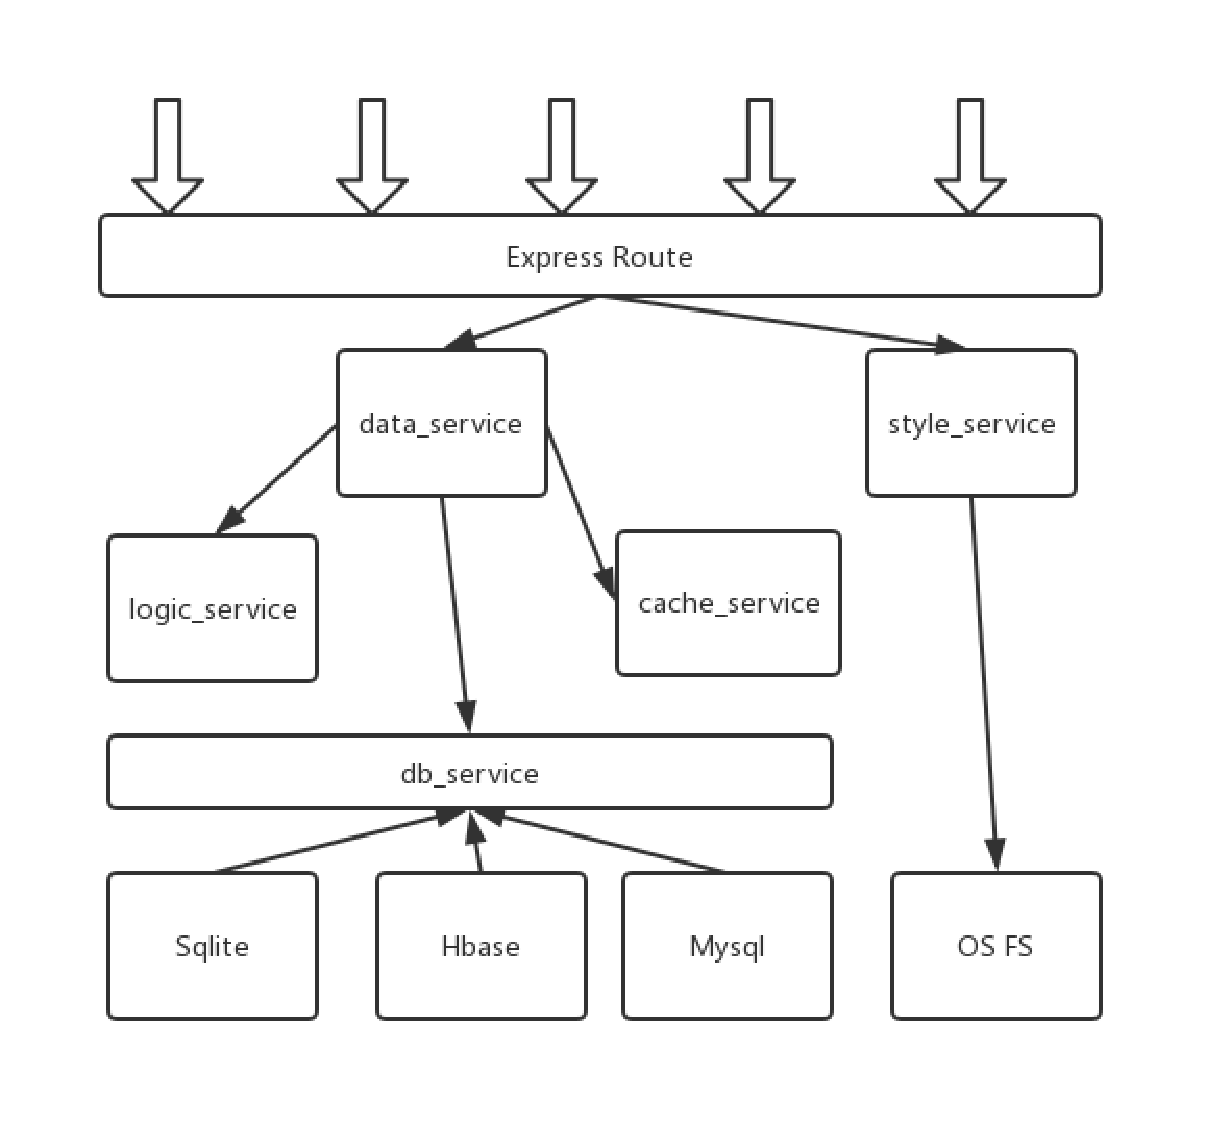
\includegraphics[width=4in]{new_FIGs/chapter4/tile-server-structure.pdf}
  \caption{tile-server整体结构图}\label{tile-server-structure}
\end{figure}

由于地图瓦片服务本身接口众多,出于篇幅考虑,本文只挑选其中比较关键,创新性较强的功能点地图局部更新功能,介绍具体实现。
\section{地图局部更新功能概述}
所谓地图局部更新,指的是一张完整地图,只更新全部地图地图的一小部分。比如中国地图中,只更新北京市地图。这一功能的价值很直观,在GTDS中很实用,而类似的开源地图瓦片服务均未提供此功能。本文根据莫卡托投影法的计算原理,实现了这一功能。

由于用户在浏览器界面上框选出来的,一定是经纬度坐标的范围。因此,该功能的输入参数应该是一个north,south,west,east四个数值组成的矩形框和对应的zoom,也就是bounding-box。所以,要想更新对应的瓦片数据,就必须首先要根据像素精度,将经纬度坐标转换为瓦片坐标,也就是对应的x,y,再将对应地图瓦片替换掉。这一过程中,为了避免歧义,需要做边界和精度的检查以及一致性的检查。
\section{地图局部更新功能流程图与代码实现}
\textbf{地图局部更新功能流程图}

\begin{figure}[H]
  \centering
  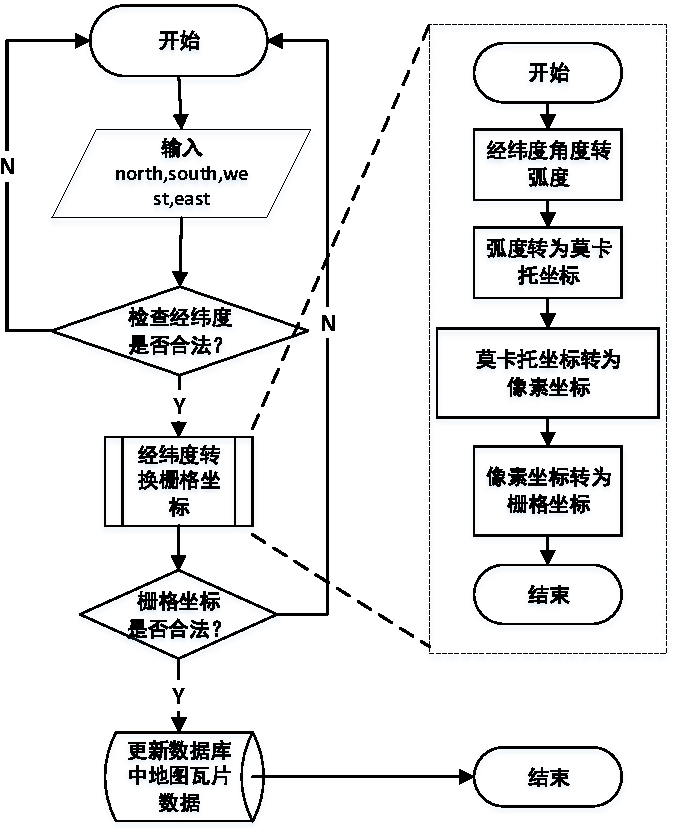
\includegraphics[width=4in,height=4in]{new_FIGs/chapter4/update_tile_1.pdf}
  \caption{地图局部更新功能流程图}\label{update_tile_1}
\end{figure}
如图\ref{update_tile_1}所示,这里值得注意的是,在流程中第二次检查,是对栅格坐标结果的检查。因为对于不同zoom,zoom值越大,地图的精度越高,更新设计的完整瓦片越多,反之则越少。那么对于那些zoom值较低的更新,其所计算出来的栅格坐标值可能不是完整的的瓦片,对于这种情况,要根据用户对精度的要求进行取舍,而取舍的前提要保证更新行为的一致性。具体可见后文。

\textbf{地图局部更新功能代码实现}

\begin{figure}[H]
  \centering
  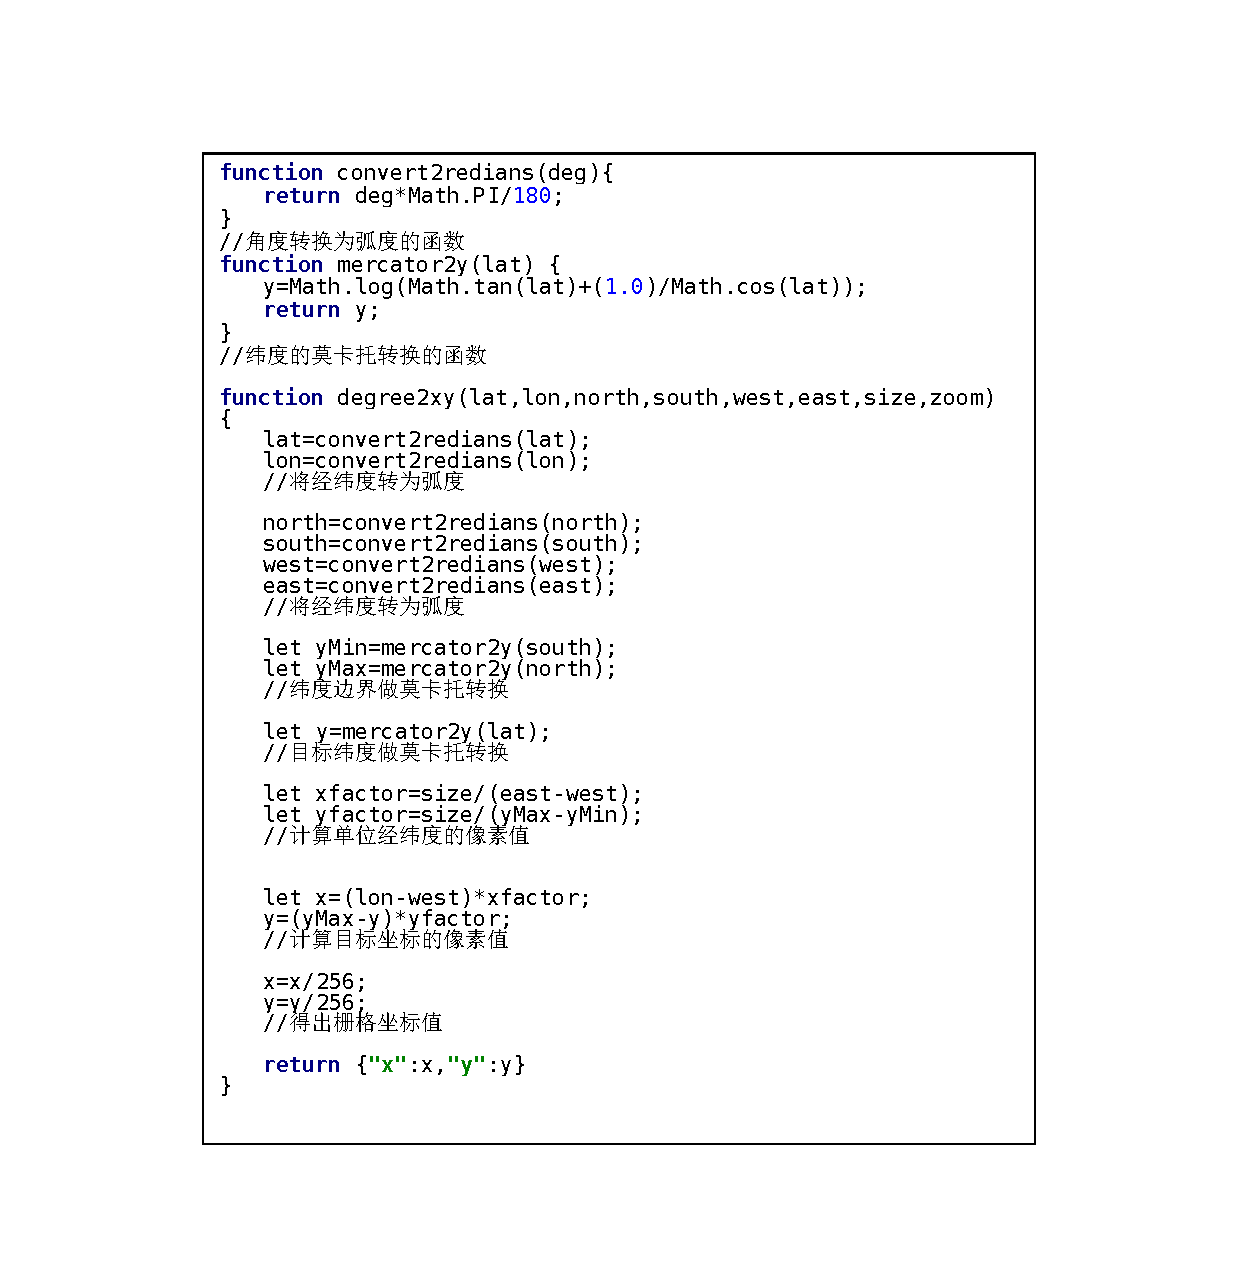
\includegraphics[width=6in]{new_FIGs/chapter4/tile_degree_compute.pdf}
  \caption{地图局部更新功能代码实现}\label{tile_degree_compute}
\end{figure}

\section{更新一致性的原理}
所谓的更新的一致性,指的是整体更新和分部分更新结果的不一致。这主要是因为单纯的栅格坐标模糊取整很可能遗漏部分栅格瓦片,导致出现更新空隙的问题。对于这个问题的解决办法,基于以下原则进行处理。

1.首先判断用户bbox更新中设置的经纬度的差值在其所设定的zoom下,是否大于等于一个Tile的边长。如果用户划定的范围太小,要求的精度太高,则直接告知用户,在当前zoom下不能更新这个bbox。如图\ref{tile_consistency0}所示,用户选定的更新范围s1的宽度小于Tile1的边长,而更新范围s2的长和宽都小于Tile2的边长。这两种情况下,都不对Tile进行更新。

\begin{figure}[H]
  \centering
  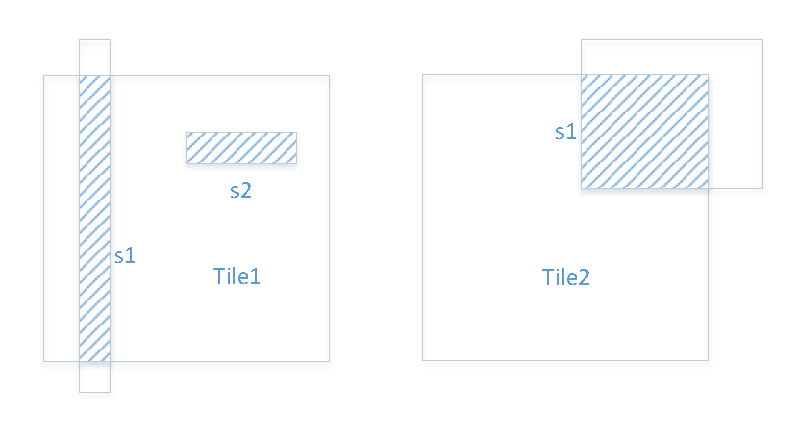
\includegraphics[width=6in,height=2.3in]{new_FIGs/chapter4/tile_consistency0.pdf}
  \caption{瓦片更新前提情况}\label{tile_consistency0}
\end{figure}

2.如果bbox的长度和宽度都大于等于Tile的边长。那么在这种情况下,对于一个Tile的bbox划分。如果划分本身是严密的,没有缝隙的。那么,1 个Tile 能且只能被划分为4个bbox.而1 个Tile的4个bbox划分中,至少有一个,其面积超过了1/4。以此作为是否更新的标准,能够保证每一个TIle至少被更新了一次,从而避免了局部更新漏掉某些Tile产生更新缝隙的问题。如图\ref{tile_consistency2}所示,图①所示,s1-s4,4块划分中,s1的面积显然大于总面积的1/4, 此时触发瓦片更新。而图②所示,s1-s4四块划分的面积都不足1/4,造成这种局面的原因是用户选定的bbox范围本身就存在间隙,没有填满整个Tile,这种情况下空隙是用户逻辑不完备造成的,瓦片数据服务不予更新。

\begin{figure}[H]
  \centering
  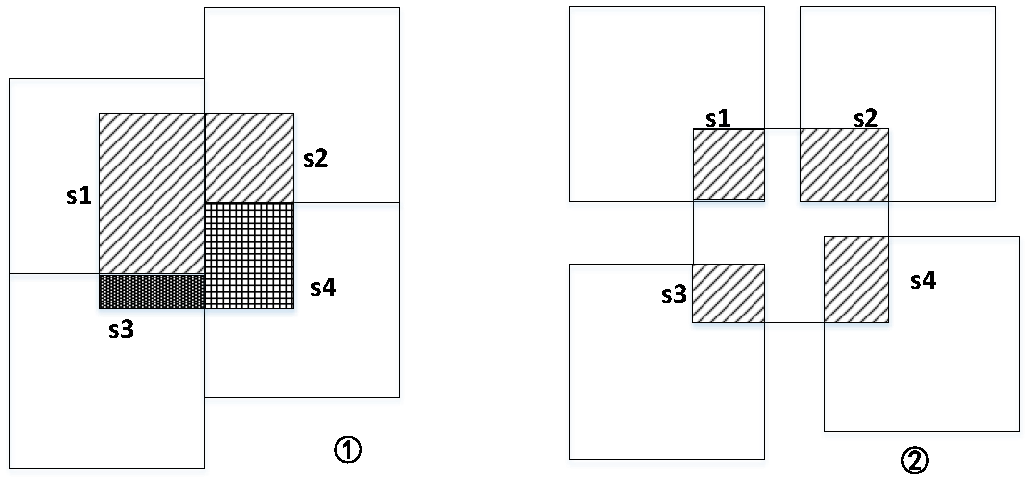
\includegraphics[width=6in,height=2.7in]{new_FIGs/chapter4/tile_consistency2.pdf}
  \caption{瓦片更新条件}\label{tile_consistency2}
\end{figure}

综上所述,本文实现的瓦片数据服务更新一致性的功能是瓦片级别的弱一致性,其依据的是用户操作本身对bbox的一致性划分。

\begin{figure}[H]
  \centering
  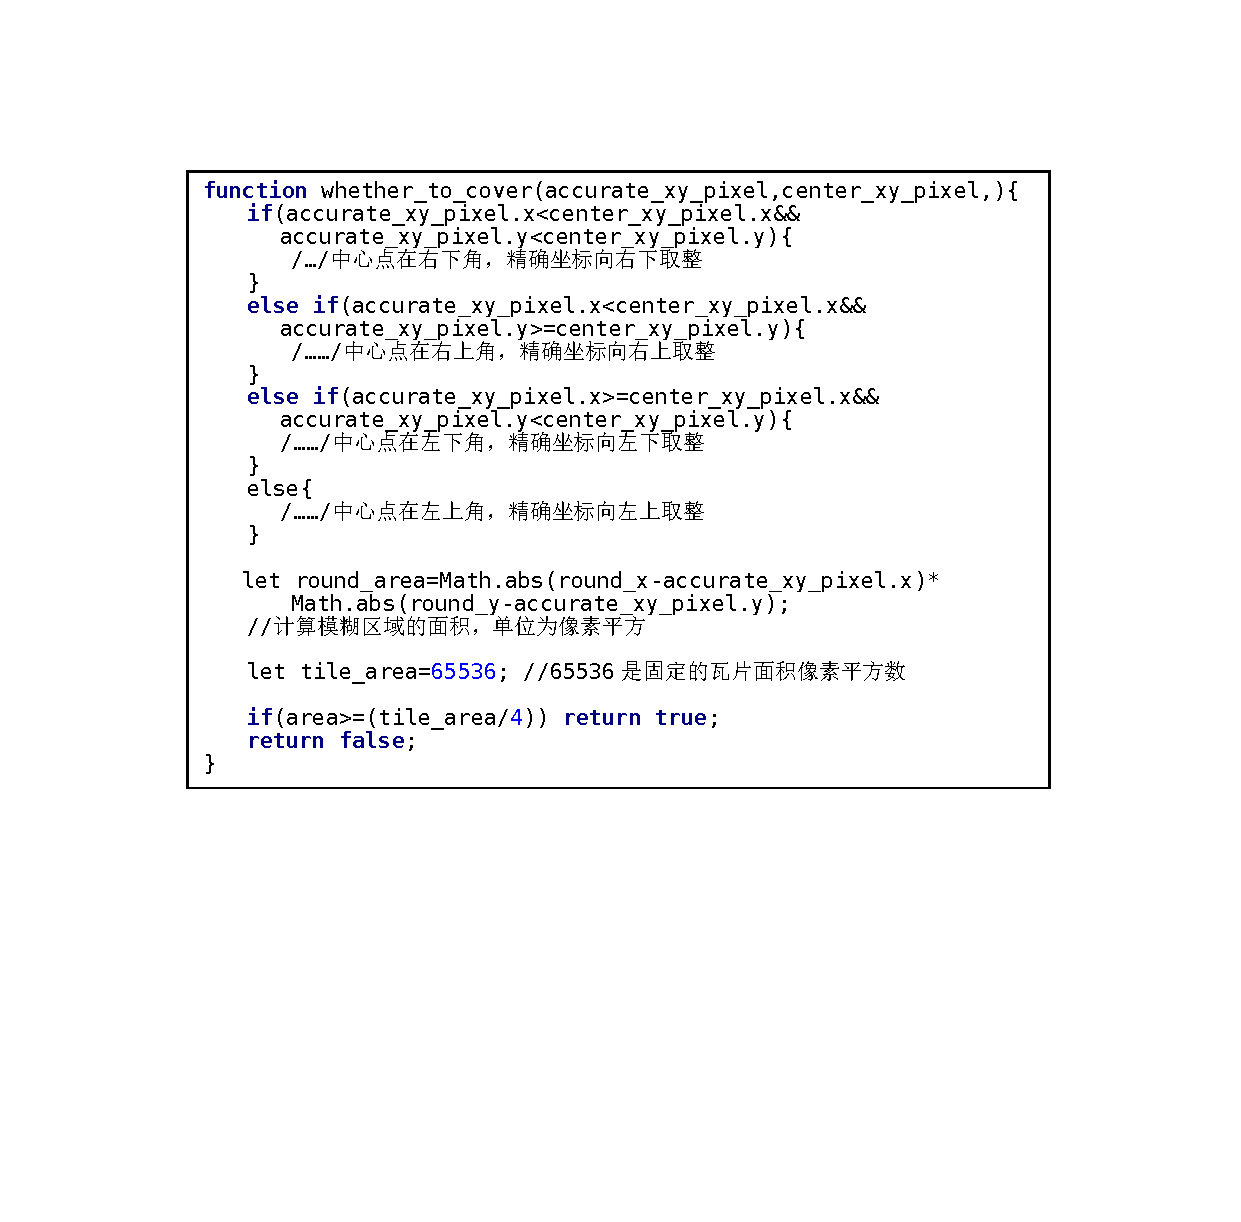
\includegraphics[width=6in,height=4in]{new_FIGs/chapter4/consistancy-code.pdf}
  \caption{判断是否覆盖当前瓦片的代码}\label{consistancy-code}
\end{figure}

\section{服务运行效果展示}
\begin{figure}[H]
  \centering
  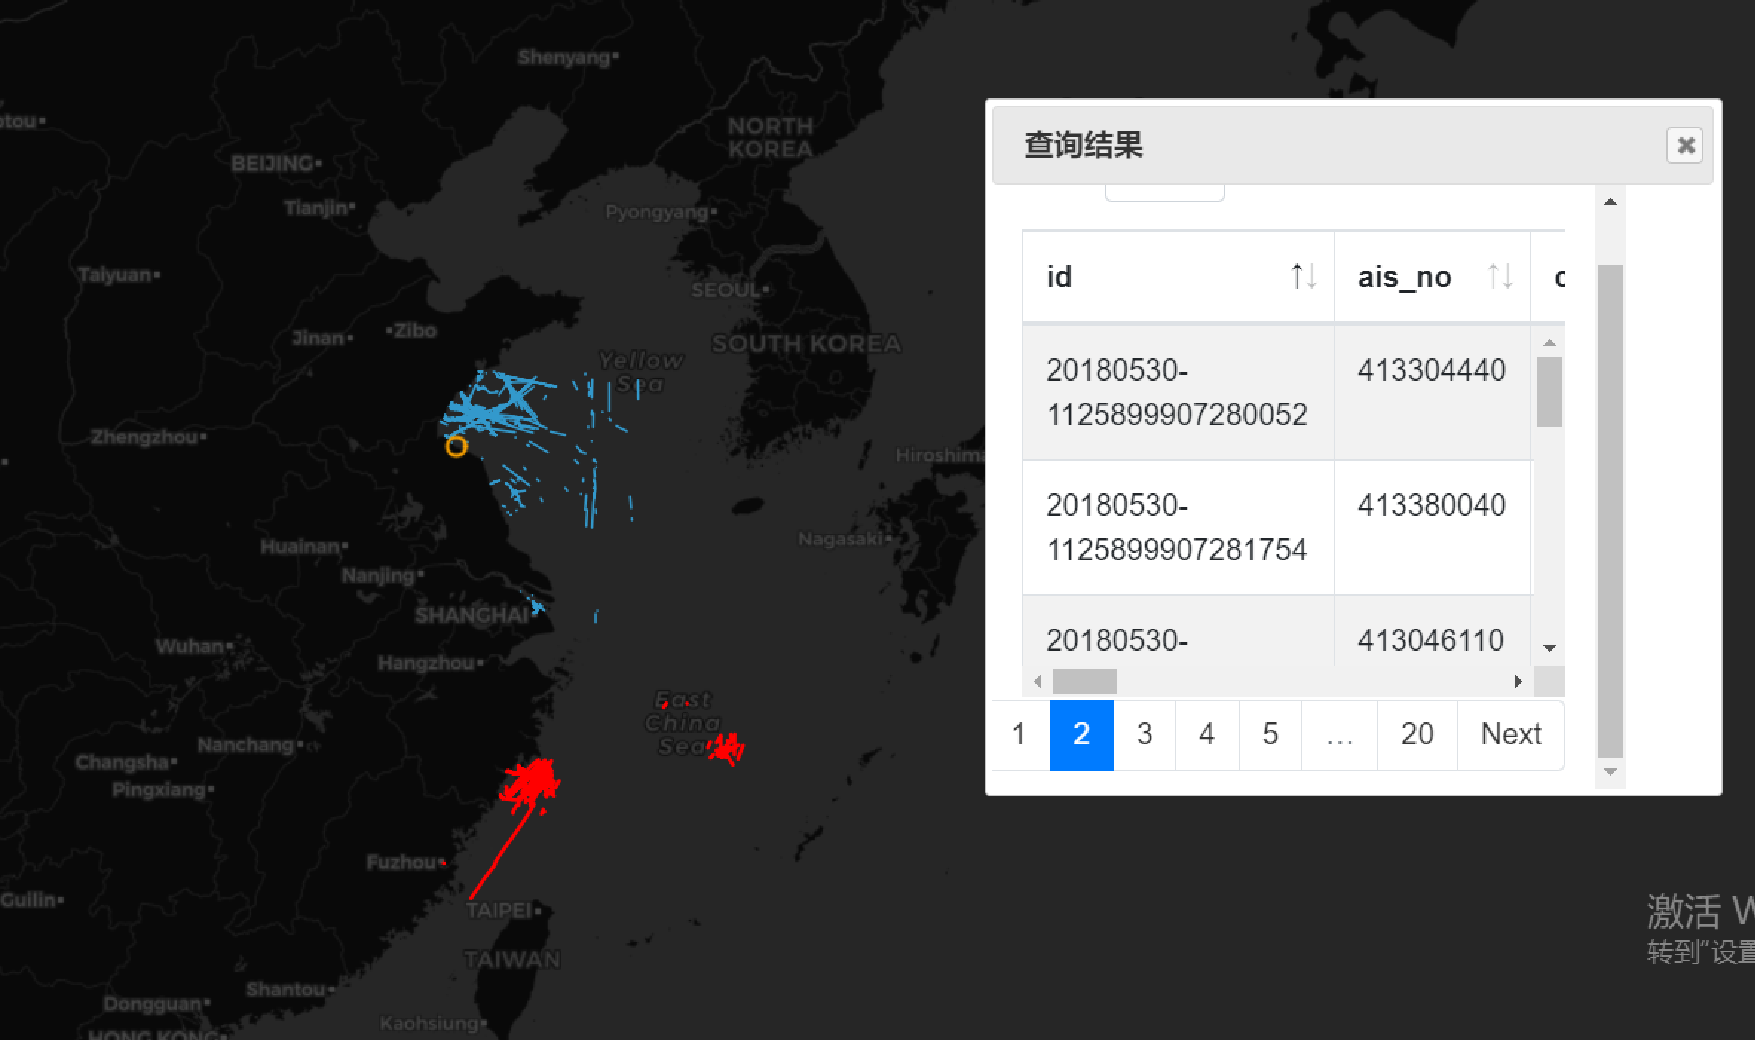
\includegraphics[width=6in]{new_FIGs/chapter5/running.pdf}
  \caption{轨迹检索运行效果}\label{running}
\end{figure}
如图\ref{running}所示,图中的地图背景为中国东海岸,两个红色群集和以浅蓝色群集构成了3个船舶轨迹的数据集合。右侧框中显示了相似检索结果,轨迹的ID 是数据采集的日期。
\section{本章总结}
本章描述了地图瓦片数据服务的详细设计和实现,主要介绍了地图瓦片数据服务的整体结构,并针对创新性较强的地图局部更新功能进行了详细设计说明。通过流程图和代码实现来说明设计和实现的思路,然后对局部更新可能出现的不一致问题给出了解决办法和原理,最后展示了系统整体运行的效果图。
